
\section{Cloud-based mobile name resolution}
%\subsection{Motivation}

%Is it possible to retrofit current DNS design to provide name resolution for 10 billion mobile hosts? 

What if DNS were to support name resolution for 10 billion mobile hosts? 

The high mobility of end hosts would require authoritative name servers to handle many orders of magnitude larger update rates of records for mobile hosts than those seen for current domain names. Organizations could either provision more resources at the authoritative name servers to handle this increase in traffic, or else outsource their DNS service to a cloud based provider. Individuals would also require an authoritative name service for their devices, and hence would likely purchase this service from a cloud provider rather than maintaining their own authoritative name servers.

Cloud based DNS services are already popular. These \emph{managed DNS providers} maintain authoritative name servers on behalf of their customers and are used by many large enterprises, e.g. Twitter uses Dyn DNS, Forbes uses UltraDNS, etc. These providers have  geo-distributed deployments at few tens of locations and achieve better performance and availability than authoritative name servers deployed at a single location. A cost associated with multiple deployments is that of keeping updated copies of the name record at every location. The pricing models of these providers already reflect this cost. Several providers offer two service-tiers with the lower-tier serving  the user from  a much smaller number of locations. The orders of magnitude higher update costs due to high mobility of end hosts would be a key concern for these providers.

We quantify the improvement in DNS lookup latency that several domains would see by switching to a managed DNS service providers. FILL IN TEXT.


Is it possible to further improve the performance? A massively geo-distributed deployment at hundreds of locations would obviously result in smaller latencies, but would also increase the associated \emph{update costs} for the provider by the same factor. Our thesis is that the update costs could be controlled by replicating a record at small number of locations, but the performance improvements resulting from a massively geo-distributed deployment still be had, if we carefully select the locations where a name record is replicated. FILL IN TEXT. This result shows that massively geo-distributed server deployments could potentially improve  performance with a better placement policy without increasing the update costs for the providers.


A fixed replication policy, e.g., replicate at all locations, or replicate at a constant number of  random locations, would be a significant handicap in  providing  a cost-effective, and high performance name resolution for all mobile hosts. A replicate-at-all-locations policy would incur excessively high update costs at every location, which would limit the number of deployment locations and keep latencies high. An alternative, i.e., replicate at a constant number random locations would result in lesser costs but would incur high latencies even with a massively geo-distributed deployment at hundreds or thousands of locations.   

To support name records for billions of mobile devices, we seek to design a massively geo-distributed system which incurs a small fraction of update costs of a replicate-at-all-locations policy but gives performance that is close to it. 


%%%%%%%%%%%%%previous version of this section v2%%%%%%%%%%%%%

\eat{
\subsection{Is DNS a cost-effective solution?}

Is it possible to retrofit current DNS design to provide name resolution for mobile hosts? What, if any, are the performance or scalability constraints that DNS would encounter?

To provide name resolution for mobile hosts, DNS would face two main challenges. First is the scale of the workload. DNS currently manages name records for 146 million domain names \cite{whois}. As the number of mobile devices already exceeds 1 billion \cite{gartner}, DNS would be expected to support name resolution for at least an order of magnitude more names that it does today. Given the success of DNS in scaling to a workload of size $10^8$, we expect that another  order of magnitude increase in workload could possibly be handled by provisioning more resources at every level of its hierarchy. 

The second challenge is that authoritative name servers would see many orders of magnitude larger update rates of records for mobile hosts than those seen for current domain names. 
This challenge too is addressable if a small number (2-3) of replicas of authoritative name servers are maintained. 
The additional update load could be supported by  provisioning more resources at authoritative name servers if necessary. To keep a small number of consistent replicas of an authoritative name server would further inflate the cost by a small factor, and hence could be supported.
%2-3, which is a manageable factor of increase in cost. Thus, for a small number of authoritative name servers, DNS appears to handle this challenge as well. 

 The  key problem with maintaining authoritative name servers at a small number of locations is that address lookups to authoritative name servers take as long as global propagation delays, i.e., hundreds of milliseconds, and result in increased connection setup times. The state-of-the-art solutions for authoritative name servers, managed DNS providers \cite{ultradns, dyndns, dnsmadeeasy}, address this problem by deploying servers at a few tens of locations globally and replicating name records from their customers at all locations.  These providers provide authoritative DNS service for  many of the top enterprises today.
 
% If these providers were to provide authoritative name service for mobile hosts, their current design makes it extremely hard for them to provide  a cost-effective, and high performance  service due to following reasons:
 
The current design of managed DNS providers makes it extremely hard for them to provide  a cost-effective, and high performance  service for all mobile hosts in the Internet. These providers would incur excessively high update cost at each location due to their policy of replicating name records at all locations. For example, processing 100M updates/sec from 10 billion mobile devices alone would require thousands of machines to be deployed at every location. This "replicate-everywhere" policy entails that the deployment consists of a small number of locations each of the size of a large data center. Thus, due to high update costs associated with adding new locations, it would be much more costly to maintain even their current deployment of tens of locations across the globe;   and  infeasible to have a massively geo-distributed deployment at hundreds or thousands of locations, e.g. Akamai's servers are deployed at more than 10000 locations, that provides small lookup latencies (few ms) to users across the globe. 

While high mobility of end-hosts makes it costlier to have more deployments, managed DNS providers do have considerable room for reducing lookup latencies with a more geo-distributed deployment of servers. We measured the address lookup latency to authoritative name servers for 318 domain names that are serviced by a leading managed DNS provider. These measurements were done from 100 PlanetLab locations by sending a total of 1000 lookups for each domain name across all locations. Figure \ref{fig:lookuplocation} shows the distribution of median lookup latencies at all locations. Lookup latency is more than 100 ms from  30\% percent of the locations. This finding suggests that the current deployment of managed DNS providers, due to a limited geo-distribution of their servers, does not fully address the problem of high lookup latencies to the authoritative name servers.



\begin{figure}
\centering
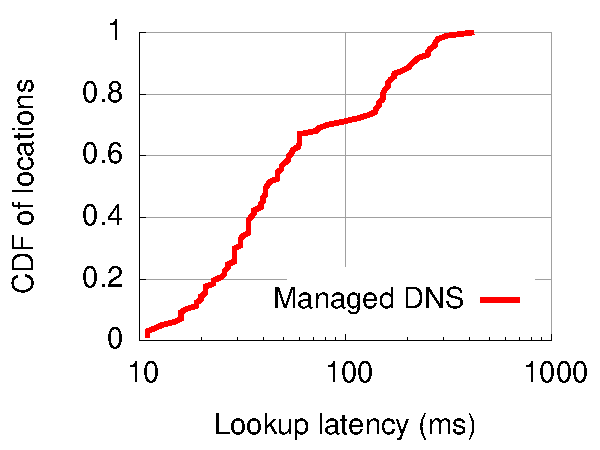
\includegraphics[scale=0.5]{graph/newgraphs/lookup-location.pdf}
\vspace{-0.1in}
\caption{Distribution of latency of lookups to authoritative name servers of a managed DNS provider from 100 Planetlab locations.}
\label{fig:lookuplocation}
\vspace{-0.1in}
\end{figure}



% from 100 PlanetLab locations to authoritative name servers  for 318 domain names that are serviced by a leading managed DNS provider (refer to Section \ref{sec:managed}). 
%This finding suggests that managed DNS providers have considerable room for reducing lookup latencies with a more geo-distributed deployment of servers.

In summary, the current DNS design could be used to provide name resolution for mobile hosts but would continue to face the problem of high lookup latency to the authoritative name servers. Having a massively geo-distributed deployment of authoritative name servers could provide low lookup latencies across the globe, but prohibitively high update costs associated with mobility makes it infeasible for managed DNS providers to support such a deployment in a cost-effective manner.
}

%
%
%
%For the name records of mobile hosts, authoritative name servers would see an update rate that is orders of magnitude higher than those of currently existing records in DNS.  over-provision authoritative name servers to solve the problem. 
%Second problem, which plagues name DNS even today is that lookups to authoritative name servers results in high latencies. 
%
%



%%%%%%%%%%%%%previous version of this section v1%%%%%%%%%%%%%

\eat{
Providing name resolution for mobile hosts would present DNS with a workload with very different characteristics than that of today's DNS.
For the name records of mobile hosts, authoritative name servers would see an update rate that is orders of magnitude higher than those of currently existing records in DNS. 
Frequent address updates by mobile hosts imply that cached addresses could be reused for much shorter durations. A record for a user that changes networks 100 times a day could be reused only for 15 minutes on average, after which a fresh name record must be fetched from the authoritative name servers. Frequent lookups to authoritative name servers, besides increasing the load on authoritative name servers, would increase connection setup time to mobile hosts. For example, if the authoritative name server is maintained at a single location, address lookups may take of the order of global propagation delays, e.g., 100s of milliseconds. Increased load of lookups and updates on authoritative name servers could be managed by provisioning more resources at authoritative name servers, but high lookup latency to authoritative name servers remains the primary problem for current DNS.
%Therefore,  is a challenge, even though provisioning  more resources at authoritative name servers could help cater to an increased load.


The state-of-the-art solutions for authoritative name servers are provided by managed DNS providers. These providers maintain servers at a few tens of locations globally and replicate name records from their customers at all locations.  These providers handle the DNS service on behalf of many of the top enterprises today. 
However, the currently available the managed DNS provider solutions have two main shortcomings: 

(1) Due to a limited geo-distribution of their servers, managed DNS providers do not fully address the problem of high lookup latencies to the authoritative name servers. We measured lookup latency to authoritative name servers for 318 domain names that are serviced by a leading managed DNS provider from 150 PlanetLab locations. Figure 1 shows the distribution of lookup latencies in our measurements. 30\% percent of lookups take more than 100 ms. 
%authoritative name servers managed DNS providers from 150 PlanetLab locations to 318 domain names in the top 10K websites as per Alexa ranking; these names are served by a leading managed DNS provider.

%For instance, to connected to a mobile host who is 10 ms away, may need a lookup that is 150 ms or even more.


(2) These providers would incur excessively high update cost at each location due to their policy of replicating name records at all locations. For example, processing 100M updates/sec from 10 billion mobile devices alone would require thousands of machines to be deployed at every location. This "replicate-everywhere" policy entails that the deployment consists of a small number of locations each of the size of a large data center. Thus, due to high update costs associated with adding new locations, it is infeasible to have a massively geo-distributed deployment at thousands of locations, e.g. Akamai has 10000 locations, that provides small lookup latencies to users across the globe. 

In summary, the current DNS design is ill-suited to provide name resolution for mobile hosts due to high lookup latencies to authoritative name servers. Having a massively geo-distributed deployment of authoritative name servers could provide low lookup latencies across the globe, but prohibitively high update costs preclude such a deployment. 
}





% current design of managed DNS providers makes it extremely hard for them to provide  a cost-effective, and high performance  service for all mobile hosts in the Internet. These providers would incur excessively high update cost at each location due to their policy of replicating name records at all locations. For example, processing 100M updates/sec from 10 billion mobile devices alone would require thousands of machines to be deployed at every location. This "replicate-everywhere" policy entails that the deployment consists of a small number of locations each of the size of a large data center. Thus, due to high update costs associated with adding new locations, it would be much more costly to maintain even their current deployment of tens of locations across the globe;   and  infeasible to have a massively geo-distributed deployment at hundreds or thousands of locations, e.g. Akamai's servers are deployed at more than 10000 locations, that provides small lookup latencies (few ms) to users across the globe. 


%\section{other stuff}
%
%
%1. high mobility ... authoritative name servers will have a very high update load
%
%2. cost advantage of a cloud service
%
%3. performance advantage of a cloud service: Managed DNS gives better performance than DNS
%
%4. is it possible to do better? yes there is room to do better than static replication policy.
%
%5. Challenge before us: system than can be massively geo-distributed, update cost that is close to static-K replication policy.
%
%
%
%Our motivation is to design a service that can support name resolution, i.e., mapping of a name to its network addresses, for every mobile device in the world. Such a service would enable any Internet host to establish connection to a mobile device.
% enable mobile-to-mobile communications, 
%
%
%
%In DNS terminology, this service plays the role of an authoritative name server -- It keeps the most up to date addresses of a device. In order to support high mobility of end hosts, the primary requirement is that this service must support many orders of magnitude higher update rates than those seen by  authoritative name servers in DNS today. 
%
%
%
%Service providers would runs this service on a cloud platform and individuals and organizations purchase this service from the for their mobile devices. We 
%
%We seek to address the concerns of a service provider who runs this service on a cloud platform 
%
%The service would be run by a provider on a cloud platform 
%
%
%
%Why should this service be run as a cloud 
%
%
%
%The alternate model, where both individuals and organizations purchase this service from a provider who is running this service in the could, is also likely to be successful given the size of this workload -- 100 M updates / sec from 10 billion devices -- and the resulting economies of scale.
%
%
%
%It is conceivable that every organization runs an independent service  service in-house,  similar to the current deployment of  authoritative name servers. The alternate model, where both individuals and organizations purchase this service from a provider who is running this service in the could, is also likely to be successful given the size of this workload -- 100 M updates / sec from 10 billion devices -- and the resulting economies of scale.
%
%However, the aggregate size of this workload -- 100 M updates / sec from 10 billion devices -- is sufficiently large to benefit from a cloud-based deployment and its resulting economies of scale.
%
%
%While it is conceivable that this service is run 
%
%While each authoritative name server is needed to add to this cost, 
%
%While it is 
%
%A highly distributed deployment 
%
%
%
%A cloud based model 
%
%A key requirement of this service is that 
%
% requirement of such a service 
%
%
%The differentiating factor between this service and 
%
%
%design a service. in DNS terminology, such as service, plays similar role  act like authoritative name service.
%
%the primary difference between this work load and workload seen by authoritative name servers today is the very high load of updates. 
%
%several models in which this service could be deployed. 
%
%each organization runs a small scale service: 
%
%each organization: It is a non-trivial workload even for a simple name service 
%
%
%
%Cloud based DNS services are already popular.
%managed dns 
%Used by large enterprises.
%
%
%Today's cloud based DNS services offer better performance.
%
%
%Is it possible to do better? for mobile workloads? yes it is.  
%
%
%Fixed replication policy: replicate-all or static-k is a limitation. replicate-all due to high cost static-k due to higher latency.
%
%
%Key challenge is the design of a distributed system whose update cost is similar to static-k but performance is close to replicate-all.
%
